% This is "sig-alternate.tex" V2.1 April 2013
% This file should be compiled with V2.5 of "sig-alternate.cls" May 2012
%
% This example file demonstrates the use of the 'sig-alternate.cls'
% V2.5 LaTeX2e document class file. It is for those submitting
% articles to ACM Conference Proceedings WHO DO NOT WISH TO
% STRICTLY ADHERE TO THE SIGS (PUBS-BOARD-ENDORSED) STYLE.
% The 'sig-alternate.cls' file will produce a similar-looking,
% albeit, 'tighter' paper resulting in, invariably, fewer pages.
%
% ----------------------------------------------------------------------------------------------------------------
% This .tex file (and associated .cls V2.5) produces:
%       1) The Permission Statement
%       2) The Conference (location) Info information
%       3) The Copyright Line with ACM data
%       4) NO page numbers
%
% as against the acm_proc_article-sp.cls file which
% DOES NOT produce 1) thru' 3) above.
%
% Using 'sig-alternate.cls' you have control, however, from within
% the source .tex file, over both the CopyrightYear
% (defaulted to 200X) and the ACM Copyright Data
% (defaulted to X-XXXXX-XX-X/XX/XX).
% e.g.
% \CopyrightYear{2007} will cause 2007 to appear in the copyright line.
% \crdata{0-12345-67-8/90/12} will cause 0-12345-67-8/90/12 to appear in the copyright line.
%
% ---------------------------------------------------------------------------------------------------------------
% This .tex source is an example which *does* use
% the .bib file (from which the .bbl file % is produced).
% REMEMBER HOWEVER: After having produced the .bbl file,
% and prior to final submission, you *NEED* to 'insert'
% your .bbl file into your source .tex file so as to provide
% ONE 'self-contained' source file.
%
% ================= IF YOU HAVE QUESTIONS =======================
% Questions regarding the SIGS styles, SIGS policies and
% procedures, Conferences etc. should be sent to
% Adrienne Griscti (griscti@acm.org)
%
% Technical questions _only_ to
% Gerald Murray (murray@hq.acm.org)
% ===============================================================
%
% For tracking purposes - this is V2.0 - May 2012

\documentclass{sig-alternate-05-2015}

\usepackage[utf8]{inputenc}
\usepackage[ngerman]{babel}

\begin{document}

% Copyright
\setcopyright{acmcopyright}
%\setcopyright{acmlicensed}
%\setcopyright{rightsretained}
%\setcopyright{usgov}
%\setcopyright{usgovmixed}
%\setcopyright{cagov}
%\setcopyright{cagovmixed}


% DOI
\doi{10.475/123_4}

% ISBN
\isbn{123-4567-24-567/08/06}

%Conference
\conferenceinfo{PLDI '13}{June 16--19, 2013, Seattle, WA, USA}

\acmPrice{\$15.00}

%
% --- Author Metadata here ---
\conferenceinfo{WOODSTOCK}{'97 El Paso, Texas USA}
%\CopyrightYear{2007} % Allows default copyright year (20XX) to be over-ridden - IF NEED BE.
%\crdata{0-12345-67-8/90/01}  % Allows default copyright data (0-89791-88-6/97/05) to be over-ridden - IF NEED BE.
% --- End of Author Metadata ---

\title{Alternate {\ttlit ACM} SIG Proceedings Paper in LaTeX
Format\titlenote{(Produces the permission block, and
copyright information). For use with
SIG-ALTERNATE.CLS. Supported by ACM.}}
\subtitle{[Extended Abstract]
\titlenote{A full version of this paper is available as
\textit{Author's Guide to Preparing ACM SIG Proceedings Using
\LaTeX$2_\epsilon$\ and BibTeX} at
\texttt{www.acm.org/eaddress.htm}}}
%
% You need the command \numberofauthors to handle the 'placement
% and alignment' of the authors beneath the title.
%
% For aesthetic reasons, we recommend 'three authors at a time'
% i.e. three 'name/affiliation blocks' be placed beneath the title.
%
% NOTE: You are NOT restricted in how many 'rows' of
% "name/affiliations" may appear. We just ask that you restrict
% the number of 'columns' to three.
%
% Because of the available 'opening page real-estate'
% we ask you to refrain from putting more than six authors
% (two rows with three columns) beneath the article title.
% More than six makes the first-page appear very cluttered indeed.
%
% Use the \alignauthor commands to handle the names
% and affiliations for an 'aesthetic maximum' of six authors.
% Add names, affiliations, addresses for
% the seventh etc. author(s) as the argument for the
% \additionalauthors command.
% These 'additional authors' will be output/set for you
% without further effort on your part as the last section in
% the body of your article BEFORE References or any Appendices.

\numberofauthors{8} %  in this sample file, there are a *total*
% of EIGHT authors. SIX appear on the 'first-page' (for formatting
% reasons) and the remaining two appear in the \additionalauthors section.
%
\author{
% You can go ahead and credit any number of authors here,
% e.g. one 'row of three' or two rows (consisting of one row of three
% and a second row of one, two or three).
%
% The command \alignauthor (no curly braces needed) should
% precede each author name, affiliation/snail-mail address and
% e-mail address. Additionally, tag each line of
% affiliation/address with \affaddr, and tag the
% e-mail address with \email.
%
% 1st. author
\alignauthor
Ben Trovato\titlenote{Dr.~Trovato insisted his name be first.}\\
       \affaddr{Institute for Clarity in Documentation}\\
       \affaddr{1932 Wallamaloo Lane}\\
       \affaddr{Wallamaloo, New Zealand}\\
       \email{trovato@corporation.com}
% 2nd. author
\alignauthor
G.K.M. Tobin\titlenote{The secretary disavows
any knowledge of this author's actions.}\\
       \affaddr{Institute for Clarity in Documentation}\\
       \affaddr{P.O. Box 1212}\\
       \affaddr{Dublin, Ohio 43017-6221}\\
       \email{webmaster@marysville-ohio.com}
% 3rd. author
\alignauthor Lars Th{\o}rv{\"a}ld\titlenote{This author is the
one who did all the really hard work.}\\
       \affaddr{The Th{\o}rv{\"a}ld Group}\\
       \affaddr{1 Th{\o}rv{\"a}ld Circle}\\
       \affaddr{Hekla, Iceland}\\
       \email{larst@affiliation.org}
\and  % use '\and' if you need 'another row' of author names
% 4th. author
\alignauthor Lawrence P. Leipuner\\
       \affaddr{Brookhaven Laboratories}\\
       \affaddr{Brookhaven National Lab}\\
       \affaddr{P.O. Box 5000}\\
       \email{lleipuner@researchlabs.org}
% 5th. author
\alignauthor Sean Fogarty\\
       \affaddr{NASA Ames Research Center}\\
       \affaddr{Moffett Field}\\
       \affaddr{California 94035}\\
       \email{fogartys@amesres.org}
% 6th. author
\alignauthor Charles Palmer\\
       \affaddr{Palmer Research Laboratories}\\
       \affaddr{8600 Datapoint Drive}\\
       \affaddr{San Antonio, Texas 78229}\\
       \email{cpalmer@prl.com}
}
% There's nothing stopping you putting the seventh, eighth, etc.
% author on the opening page (as the 'third row') but we ask,
% for aesthetic reasons that you place these 'additional authors'
% in the \additional authors block, viz.
\additionalauthors{Additional authors: John Smith (The Th{\o}rv{\"a}ld Group,
email: {\texttt{jsmith@affiliation.org}}) and Julius P.~Kumquat
(The Kumquat Consortium, email: {\texttt{jpkumquat@consortium.net}}).}
\date{30 July 1999}
% Just remember to make sure that the TOTAL number of authors
% is the number that will appear on the first page PLUS the
% number that will appear in the \additionalauthors section.

\maketitle
\begin{abstract}
This paper provides a sample of a \LaTeX\ document which conforms,
somewhat loosely, to the formatting guidelines for
ACM SIG Proceedings. It is an {\em alternate} style which produces
a {\em tighter-looking} paper and was designed in response to
concerns expressed, by authors, over page-budgets.
It complements the document \textit{Author's (Alternate) Guide to
Preparing ACM SIG Proceedings Using \LaTeX$2_\epsilon$\ and Bib\TeX}.
This source file has been written with the intention of being
compiled under \LaTeX$2_\epsilon$\ and BibTeX.

The developers have tried to include every imaginable sort
of ``bells and whistles", such as a subtitle, footnotes on
title, subtitle and authors, as well as in the text, and
every optional component (e.g. Acknowledgments, Additional
Authors, Appendices), not to mention examples of
equations, theorems, tables and figures.

To make best use of this sample document, run it through \LaTeX\
and BibTeX, and compare this source code with the printed
output produced by the dvi file. A compiled PDF version
is available on the web page to help you with the
`look and feel'.
\end{abstract}


%
% The code below should be generated by the tool at
% http://dl.acm.org/ccs.cfm
% Please copy and paste the code instead of the example below. 
%
\begin{CCSXML}
<ccs2012>
 <concept>
  <concept_id>10010520.10010553.10010562</concept_id>
  <concept_desc>Computer systems organization~Embedded systems</concept_desc>
  <concept_significance>500</concept_significance>
 </concept>
 <concept>
  <concept_id>10010520.10010575.10010755</concept_id>
  <concept_desc>Computer systems organization~Redundancy</concept_desc>
  <concept_significance>300</concept_significance>
 </concept>
 <concept>
  <concept_id>10010520.10010553.10010554</concept_id>
  <concept_desc>Computer systems organization~Robotics</concept_desc>
  <concept_significance>100</concept_significance>
 </concept>
 <concept>
  <concept_id>10003033.10003083.10003095</concept_id>
  <concept_desc>Networks~Network reliability</concept_desc>
  <concept_significance>100</concept_significance>
 </concept>
</ccs2012>  
\end{CCSXML}

\ccsdesc[500]{Computer systems organization~Embedded systems}
\ccsdesc[300]{Computer systems organization~Redundancy}
\ccsdesc{Computer systems organization~Robotics}
\ccsdesc[100]{Networks~Network reliability}


%
% End generated code
%

%
%  Use this command to print the description
%
\printccsdesc

% We no longer use \terms command
%\terms{Theory}

\keywords{ACM proceedings; \LaTeX; text tagging}

\section{Introduction}

%\documentclass[10pt,a4paper,twocolumn]{article}
%\usepackage[utf8]{inputenc}
%\usepackage[ngerman]{babel}
%\setlength{\parindent}{0cm}
%\usepackage[colorlinks=true, urlcolor=black]{hyperref}
%\usepackage{graphicx}
%\begin{document}
	
% TODO: KDE Plasma detailierter Beschreiben
% TODO: Ein Teil / ein Subproject detailliert Beschreiben (Analyse mit Tool [cppdepend?])
	
\section{KDE Architecture}
Im Folgenden wird nun die Architektur der vom Team des KDE Projekts entwickelten KDE Software Compilation (KDE SC) vorgestellt. Der wohl bekannteste Teil der KDE Software Compilation ist die Desktop Umgebung KDE Plasma. Dazu kommt eine große Anzahl an Anwendungen die KDE Applications. Diese werden vor allem in Verbindung mit KDE Plasma genutzt können aber auch unabhängig davon verwendet werden. Der dritte Bestandteil der KDE Software Compilation heißt KDE Frameworks und stellt eine Sammlung von Bibliotheken dar. Diese enthalten häufig benötigte Funktionen und machen es somit einfacher KDE Software zu entwickeln. Außerdem wird so das ständige neu entwickeln grundlegender Funktionen verhindert. Wichtig ist in diesem Zusammenhang auch die Qt Library die zwar nicht direkt zum KDE Projekt gehört aber eng mit dem KDE Projekt verbunden ist da Qt als Basis für die Entwicklung verwendet wird.
Qt (http://www.qt.io/) ist im wesentlichen eine C++-Klassenbibliothek für die plattformübergreifende Programmierung grafischer Benutzeroberflächen die viele für die Entwicklung hilfreiche Funktionen bietet.
%\url{https://en.wikipedia.org/wiki/Qt_(software)}
%\url{http://www.qt.io/}
Auf Anwenderebene sind also die KDE Applications und KDE Plasma die auf die KDE Framworks und Qt aufbauen wie auch in Abbildung \ref{fig:kde_overview} dargestellt.
\begin{figure}[h]
\centering
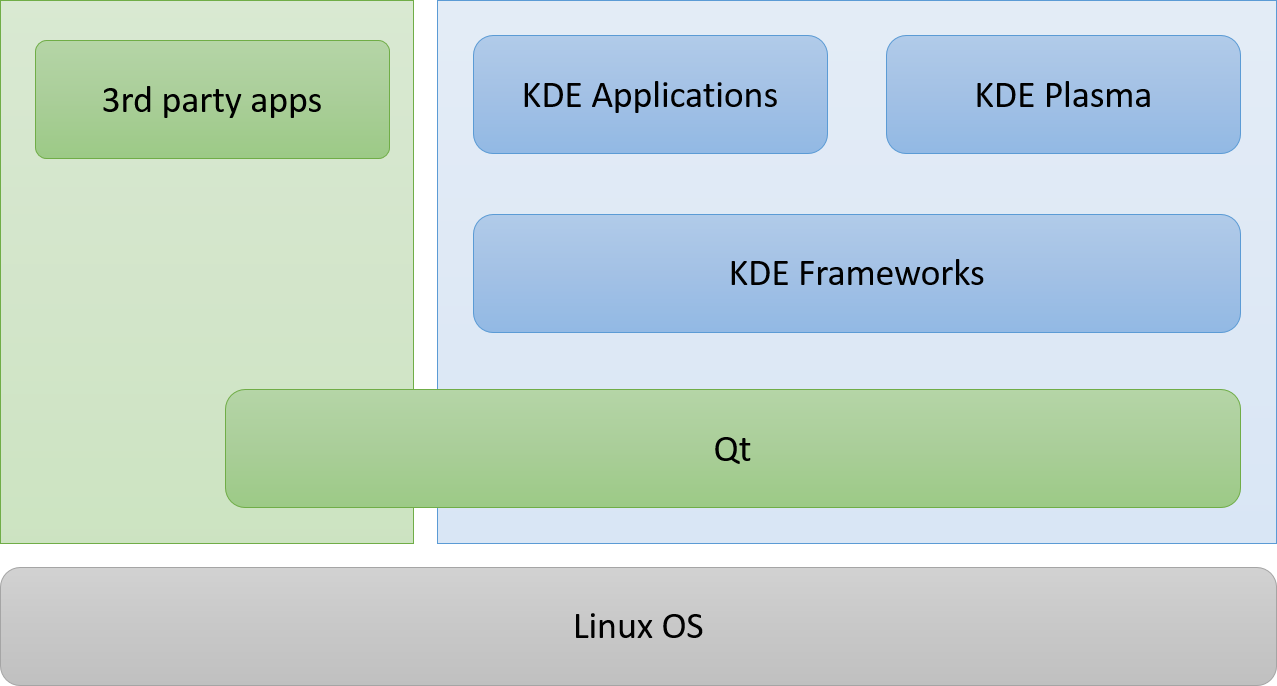
\includegraphics[width=0.9\columnwidth]{images/KDE_Aufbau.png}
\caption{KDE Übersicht}
\label{fig:kde_overview}
\end{figure}

\subsection{KDE Frameworks 5}
Das Ziel des unter der LGPL stehenden und vor allem in C++ und C entwickelten KDE Frameworks ist die Modularisierung. Aufbauend auf das als Basis genutzte Qt 5 stellt das aktuelle KDE Frameworks 5 grundlegende und für viele Anwendungsfälle nützliche Funktionen wie z.B. extra UI Elemente, Rechtschreibprüfung, usw. zu Verfügung. KDE Frameworks stellt somit durch seine verschiedenen Bibliotheken die Basis für KDE Plasma und KDE Applications dar und vereinfacht die Entwicklung, da auf erprobte Implementierungen zurückgriffen werden kann und unnötiges für jede Software neu entwickeln verhindert wird. Das KDE Frameworks 5 besteht dazu aus rund 60 einzelnen Bibliotheken mit verschiedenen Abhängigkeiten untereinander die möglichst Plattform unabhängig gehalten sind und versuchen so wenig wie möglich zusätzliche Abhängigkeiten zu verursachen. Für eine bessere Übersicht welche Abhängigkeiten existieren erfolgt dabei eine Einteilung ist nach "'Tier"' und "'Categorie"' die im Folgenden auch noch detaillierter vorgestellt wird. Abbildung \ref{fig:kde_frameworks} gibt einen groben Überblick für die Bestandteile der KDE Frameworks 5 und zu welchen "'Tier"' sie gehören.
%\url{https://dot.kde.org/2013/09/25/frameworks-5}
%https://www.kde.org/ https://dot.kde.org/ http://api.kde.org/

%\url{https://dot.kde.org/2014/01/07/frameworks-5-tech-preview}
%\url{https://dot.kde.org/sites/dot.kde.org/files/kf5_big_0.png}
\begin{figure}[h]
	\centering
	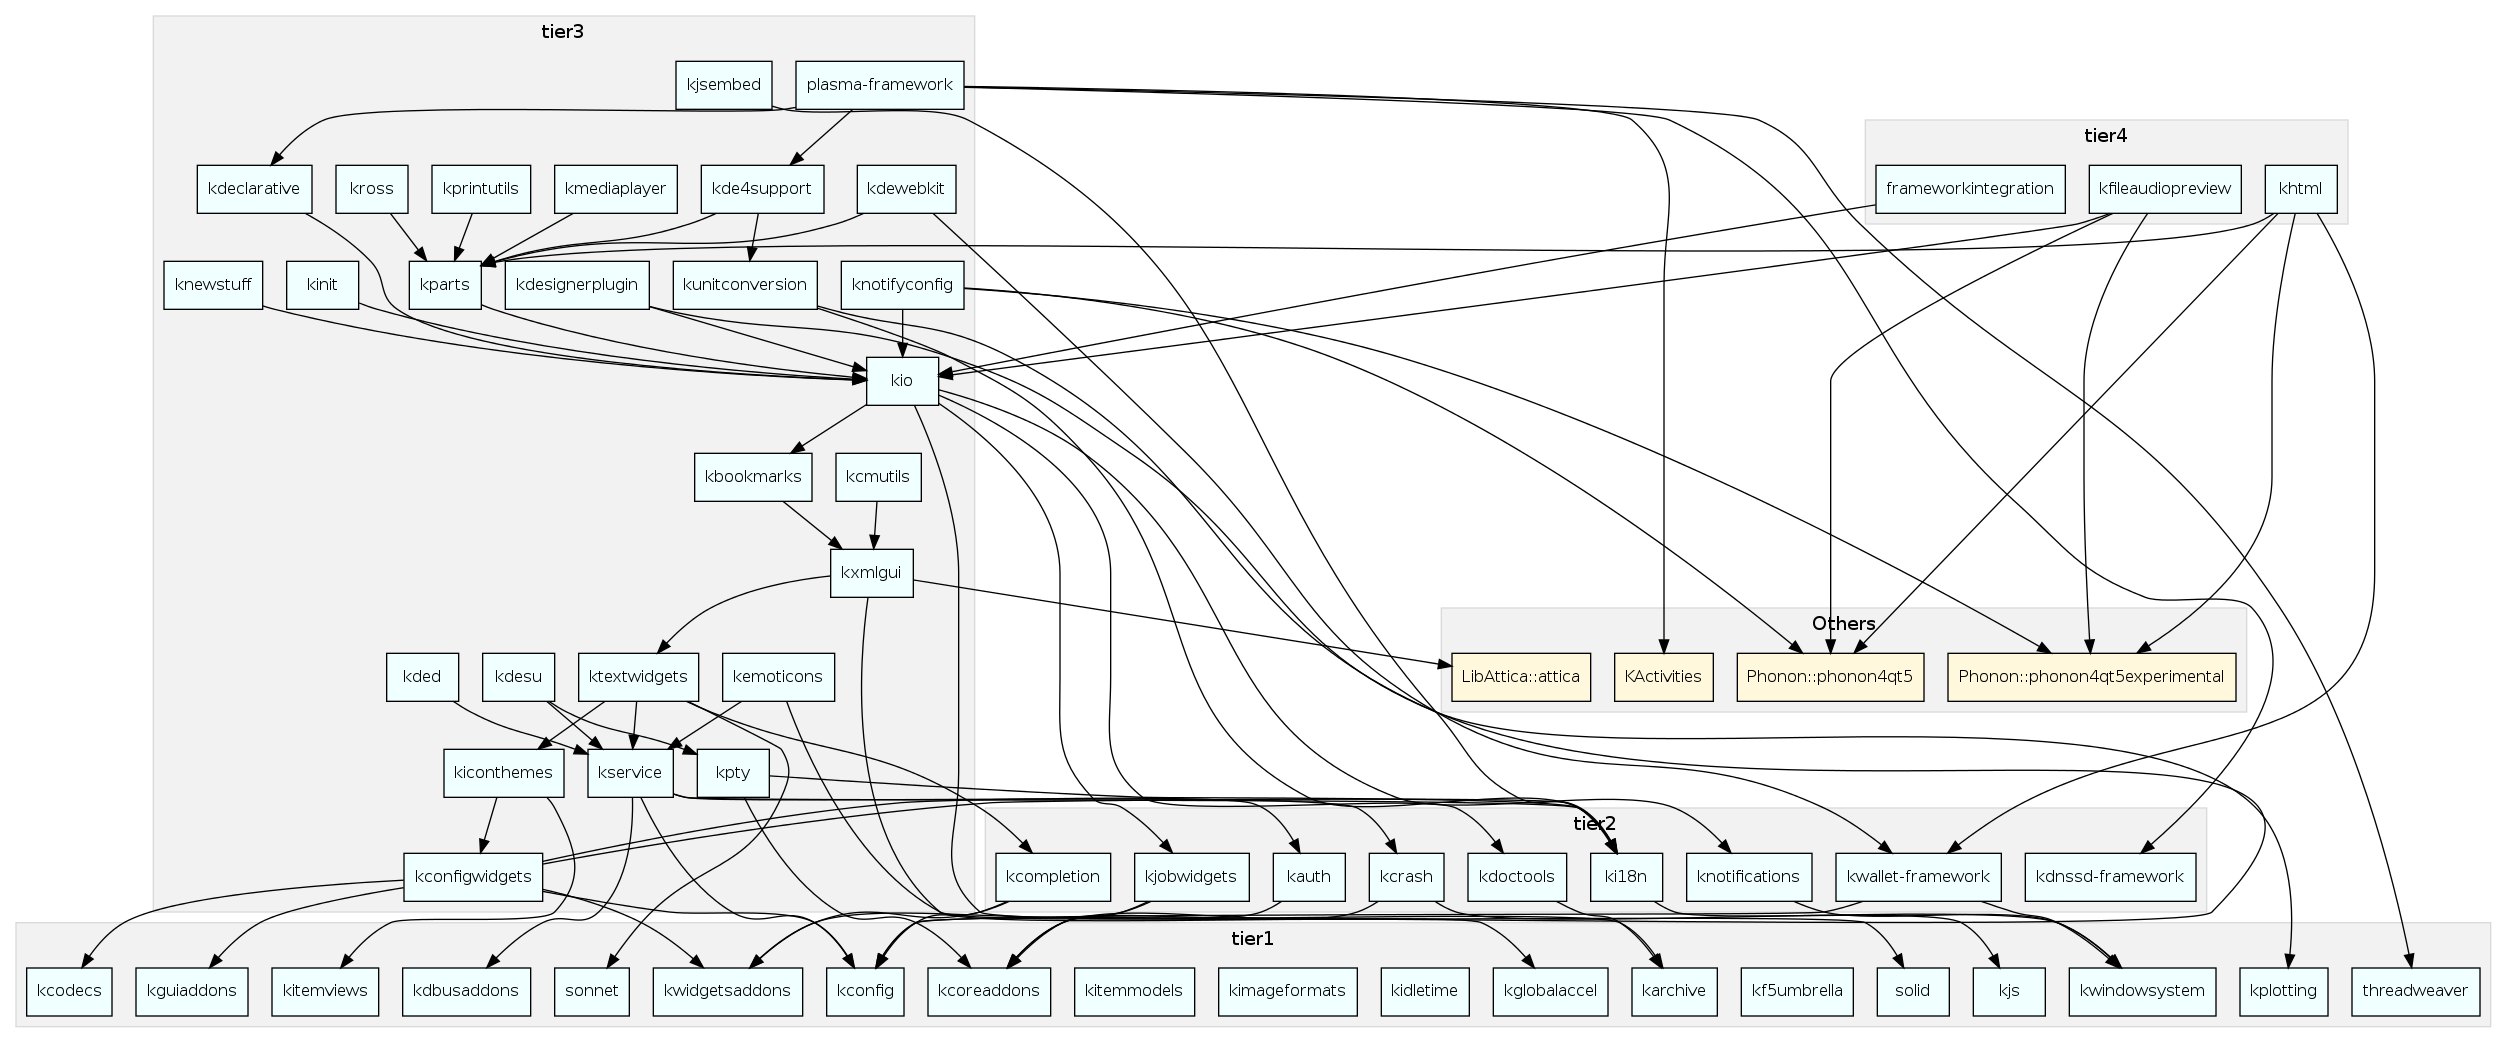
\includegraphics[width=\columnwidth]{images/kf5_big_0.png}
	\caption{KDE Frameworks}
	\label{fig:kde_frameworks}
\end{figure}

Ziel der Aufteilung in viele einzelne in KDE Frameworks gebündelte Bibliotheken ist dabei dass es leichter möglich wird nur auf Teile der KDE Frameworks aufzubauen.
Die vielen einzelnen Bibliotheken von denen immer nur die benötigen verwendet werden ist dabei eine noch recht neue für die Architektur der Software sehr wichtige Entwicklung die erst mit KDE Frameworks 5 im Dezember 2013 eingeführt wurde. KDE Frameworks in Version 4 trug noch den Namen KDE Platfrom baute noch auf Qt 4 und war im Prinzip nur eine einzige große KDElibs Library wie sie schon in den Versionen davor existierte.
%\url{https://en.wikipedia.org/wiki/File:Evolution_and_development_of_KDE_software.svg}
\begin{figure}[h]
\centering
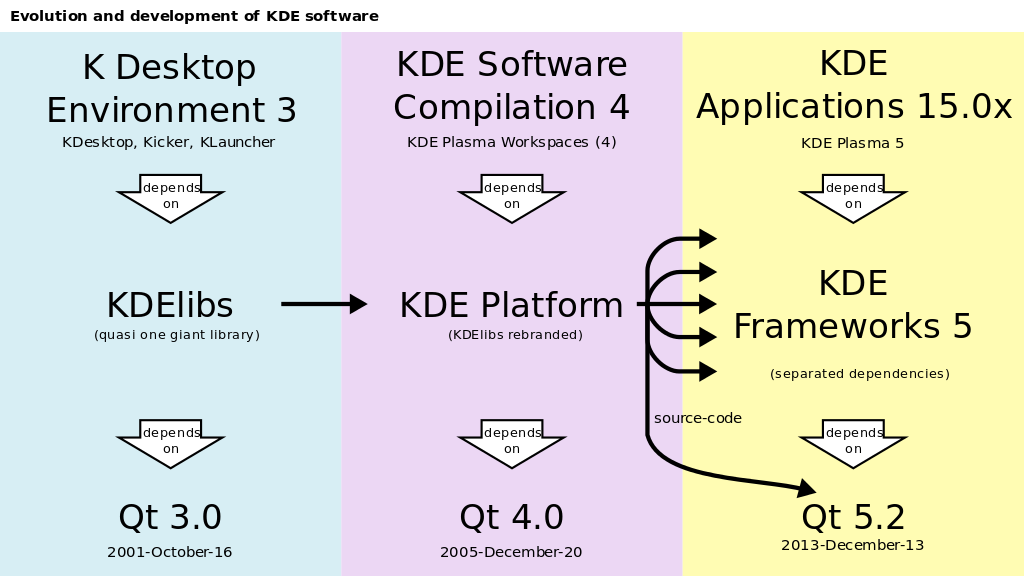
\includegraphics[width=\columnwidth]{images/Evolution_and_development_of_KDE_software}
\caption{KDE Frameworks}
\label{fig:Evolution_and_development_of_KDE_software}
\end{figure}

Große umbauten auf KDE Frameworks Ebene wie z.B. von Version 4 auf 5 beeinflussen allerdings alle darauf aufbauende Software weshalb verschiedene KDE Frameworks Versionen parallel von verschieden Anwendungen genutzt werden können, so dass Anwendungen die darauf aufbauen in Ruhe beim erscheinen einer neuen Version auf diese portiert werden können. Major Releases (Versionsnummer X.0) brechen dabei die Abwärtskompatibilität und steigen auch auf die nächste große Qt Version um. Minor Veröffentlichungen (X.1, X.2, ...) hingegen garanteiren Source und Binär Kompatibilität und sind meist kleine Weiterentwicklungen, Verbesserungen und vor allem Fehlerkorrekturen.

%https://www.kde.org/developerplatform/
Bekannte Frameworks aus den KDE Framworks 5 sind z.B. Sonnet eine Rechtschreib- und Grammatikprüfung, KHTML eine HTML und JS Library, Solid eine Hardware und Network Abstraktion und Phonon ein Multimedia Framework. Eine Vollständige Liste ist in der online API Dokumentation zu finden.

Die KDE Frameworks 5 haben dabei eine klare Dependency Struktur die in "'Categorie"' und "'Tier"' einteilt. Dies hilft den Überblick zu behalten welche Abhängigkeiten der Einsatz eines bestimmten Framework mit sich bringt. In der online API Dokumentation ist deshalb auch eine Zuordnung der Farmeworks zu den Tiers verfügbar.
%\url{https://dot.kde.org/2013/09/25/frameworks-5}
%\url{http://api.kde.org/frameworks-api/frameworks5-apidocs/}

Die Einteilung "'Categories"' bezieht sich dabei auf Laufzeit-Abhängigkeiten:
\begin{itemize}
\setlength\itemsep{0em}
\item Functional: Auf Qt aufbauend und ohne weitere Laufzeit-Abhängigkeiten z.B. KArchive, KPlotting, Threadweaver, KConfig, KCoreAddons

\item Integration: Mit optionalen Laufzeit-Abhängigkeiten für Integration bzw. Kompatibilität mit Betriebssystem/Plattform darunter z.B. Sonnet, Solid

\item Solutions: Haben gewollt Laufzeit-Abhängigkeiten um sich damit ergebende Vorteile nutzen zu können z.B. KIO, KService
\end{itemize}

Die Einteilung in "'Tiers"' bezieht sich auf Compile-Zeit Abhängigkeiten:
\begin{itemize}
\setlength\itemsep{0em}
\item Tier 1: Keine Abhängigkeiten innerhalb KDE Frameworks, nur Ot und andere kleine Abhänglichkeiten  checkerso dass eine einfach Verwendung in einem Qt Projekt möglich ist. 

\item Tier 2: Dürfen auf Tier 1 Frameworks aufbauen haben aber weiterhin einfach zu verwaltende Abhängigkeiten.

\item Tier 3: Dürfen auf Tier 3 Farmworks genauso wie Tier 2 und Tier 1 Frameworks aufbauen und haben somit oft schon komplexere Abhängigkeiten.

\item Tier 4: Für Anwendungsentwickler unwichtig vor allem Frameworks zur Integration. 
\end{itemize}

Jedes Framework lässt sich somit klar einordnen. Außerdem gibt es eine vom KDE Projekt erstelle Tier/Categorie Matrix (siehe Abbildung \ref{fig:kde_matrix}) die verschieden sich damit ergebenden Kombinationen und Abhängigkeiten Zeigt.

%\url{https://dot.kde.org/sites/dot.kde.org/files/kf5_no_tier4_big.png}
\begin{figure}[h]
	\centering
	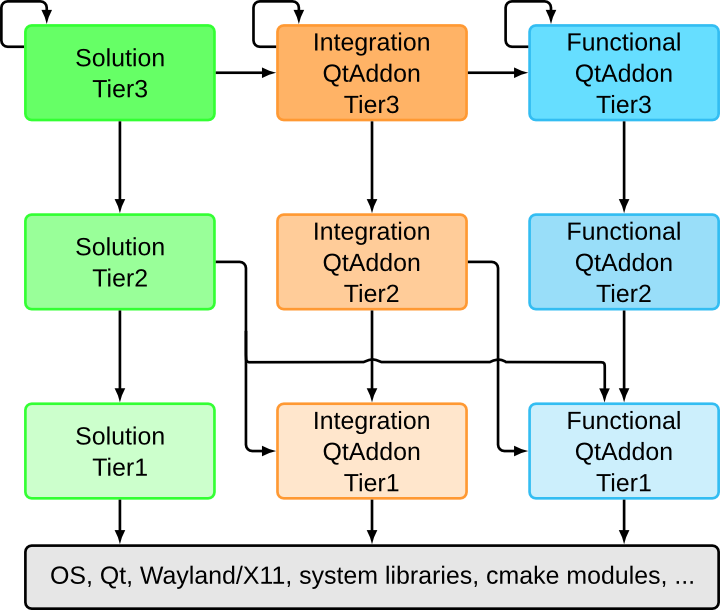
\includegraphics[width=0.9\columnwidth]{images/kf5_no_tier4_big.png}
	\caption{KDE Tier/Categorie Matrix}
	\label{fig:kde_matrix}
\end{figure}

\subsection{KDE Plasma 5}
KDE Plasma 5 stellt die bekannte für Linuxsysteme entwickelten Arbeitsplatzumgebung des KDE Projekts dar. Aufbauend auf Qt 5 und KDE Frameworks 5 findet die Entwicklung vor allem mit C++ und QML statt. 

\url{https://en.wikipedia.org/wiki/KDE_Plasma_5}
\url{http://www.heise.de/open/artikel/Plasma-5-Der-KDE-Desktop-in-neuem-Glanz-2260451.html}

// TODO: Details zur Architektur (Mit Tool wenn es sich anbietet sonst für ein einfacheres Beispiel aus dem nächsten Abschnitt)

\subsection{KDE Applications 15.12}
Viele einzelne Anwendungen die zum KDE Projekt gehören werden unter den KDE Applications zusammengefasst. Das KDE Projekt Teil die über hundert Anwendungen deshalb zur besseren Übersicht deswegen die die Kategorien Development, Education, Games, Graphics, Internet, Multimedia, Office, System und Utilities ein. Die verschieden Anwendungen der KDE Applications bauen wie KDE Plasma auf Qt und KDE Frameworks auf. Davon Abgesehen sind die einzelnen Anwendungen aber relativ unabhängig vom gesamt Projekt gehalten weshalb auch die Architektur der einzelnen Programme betreffende Entscheidungen variieren. 

// TODO: Eventuell ein Beispiel detaillierter

\url{https://en.wikipedia.org/wiki/KDE_Applications}

%\end{document}

\section{Conclusions}
This paragraph will end the body of this sample document.
Remember that you might still have Acknowledgments or
Appendices; brief samples of these
follow.  There is still the Bibliography to deal with; and
we will make a disclaimer about that here: with the exception
of the reference to the \LaTeX\ book, the citations in
this paper are to articles which have nothing to
do with the present subject and are used as
examples only.
%\end{document}  % This is where a 'short' article might terminate

%ACKNOWLEDGMENTS are optional
\section{Acknowledgments}
This section is optional; it is a location for you
to acknowledge grants, funding, editing assistance and
what have you.  In the present case, for example, the
authors would like to thank Gerald Murray of ACM for
his help in codifying this \textit{Author's Guide}
and the \textbf{.cls} and \textbf{.tex} files that it describes.

%
% The following two commands are all you need in the
% initial runs of your .tex file to
% produce the bibliography for the citations in your paper.
\bibliographystyle{abbrv}
\bibliography{sigproc}  % sigproc.bib is the name of the Bibliography in this case
% You must have a proper ".bib" file
%  and remember to run:
% latex bibtex latex latex
% to resolve all references
%
% ACM needs 'a single self-contained file'!
%
%APPENDICES are optional
%\balancecolumns
\appendix
%Appendix A
\section{Headings in Appendices}
The rules about hierarchical headings discussed above for
the body of the article are different in the appendices.
In the \textbf{appendix} environment, the command
\textbf{section} is used to
indicate the start of each Appendix, with alphabetic order
designation (i.e. the first is A, the second B, etc.) and
a title (if you include one).  So, if you need
hierarchical structure
\textit{within} an Appendix, start with \textbf{subsection} as the
highest level. Here is an outline of the body of this
document in Appendix-appropriate form:
\subsection{Introduction}
\subsection{The Body of the Paper}
\subsubsection{Type Changes and  Special Characters}
\subsubsection{Math Equations}
\paragraph{Inline (In-text) Equations}
\paragraph{Display Equations}
\subsubsection{Citations}
\subsubsection{Tables}
\subsubsection{Figures}
\subsubsection{Theorem-like Constructs}
\subsubsection*{A Caveat for the \TeX\ Expert}
\subsection{Conclusions}
\subsection{Acknowledgments}
\subsection{Additional Authors}
This section is inserted by \LaTeX; you do not insert it.
You just add the names and information in the
\texttt{{\char'134}additionalauthors} command at the start
of the document.
\subsection{References}
Generated by bibtex from your ~.bib file.  Run latex,
then bibtex, then latex twice (to resolve references)
to create the ~.bbl file.  Insert that ~.bbl file into
the .tex source file and comment out
the command \texttt{{\char'134}thebibliography}.
% This next section command marks the start of
% Appendix B, and does not continue the present hierarchy
\section{More Help for the Hardy}
The sig-alternate.cls file itself is chock-full of succinct
and helpful comments.  If you consider yourself a moderately
experienced to expert user of \LaTeX, you may find reading
it useful but please remember not to change it.
%\balancecolumns % GM June 2007
% That's all folks!
\end{document}
